%告知 CTeX 这个文件是用 UTF-8 编码
% !Mode:: "TeX:UTF-8"

%使用 pdflatex
%!TEX program = pdflatex


\documentclass[12pt,a4paper]{article}
%正文字体大小为12pt, 页面规格是A4, 使用article文档格式

\usepackage[utf8]{inputenc}
%作用是inputenc用来识别输入编码

\usepackage[left=2.2cm,right=2.2cm,top=3cm,bottom=2.5cm]{geometry}
%latex设置页面边距,页面大小,页边距

\usepackage{mathtools}
%数学公式扩展宏包,提供了公式编号定制和更多的符号、矩阵等

\usepackage{booktabs}  
%booktabs宏包画三线表,线条精细可变

\usepackage{graphicx} 
%支持插图

\usepackage{listings}
%提供了排版关键字高亮的代码环境 lslisting 以及对版式的自定义。
%类似宏包有minted



\lstset{%使用\lstset{}进行代码环境的设置
backgroundcolor=\color{cyan!10},%% 选择代码背景,必须加上\ usepackage {color}或\ usepackage {xcolor}.
basicstyle=\ttfamily, % 设置代码字号.
numbers=left,% 给代码添加行号,可取值none, left, right.
numberstyle=\scriptsize %小六号 \scriptsize
% numberstyle=\tiny\color{mygray}, % 行号的字号和颜色
}

\usepackage{fancyhdr}
%修改页眉页脚格式,令页眉页脚可以左对齐、居中、右对齐

\usepackage{tikz}%以 TikZ 为基础提供排版样式丰富的彩色盒子的功能
\usepackage[europeanresistors,americaninductors]{circuitikz}
%欧式电阻,美式电感

\usepackage{indentfirst} %令章节标题后的第一段首行缩进
\usepackage[wby]{callouts}

\lstdefinestyle{mystyle}{
    backgroundcolor=\color{white},  %背景颜色 
    commentstyle=\color{codegreen}, %注释风格
    keywordstyle=\color{magenta},   %关键字风格 红紫色
    numberstyle=\tiny\color{codegray},
    stringstyle=\color{codepurple},
    basicstyle=\footnotesize\ttfamily,breaklines=true,
    %设置代码的大小  选择一种等宽(“打字机”)字体族  对过长的代码自动换行  
    breakatwhitespace=false, %空格中断
    xleftmargin=20pt, %x左边框
    xrightmargin=20pt,%x右边框       
    breaklines=true,  %代码过长则换行               
    captionpos=b,     % 设置标题位置.               
    keepspaces=true,  % 保留空格    有助于保持代码的缩进 possibly needs columns=flexible           
    numbers=left,     % 给代码添加行号,可取值none, left, right.                   
    numbersep=5pt,    % 设置行号与代码之间的间隔              
    showspaces=false, % 显示每个地方添加特定下划线的空格; 覆盖了'showtringspaces'               
    showstringspaces=false, % 仅在字符串中允许空格
    showtabs=false,   % 在字符串中显示添加特定下划线的制表符               
    tabsize=2,        % 将默认tab设置为2个空格  
    framextopmargin=50pt,%代码区定框
    frame=bottomline,   %代码区底部
    basicstyle=\footnotesize\ttfamily,  % 设置代码字号
    language=Octave     % 使用的语言
}
\usepackage{ulem}%提供排版可断行下划线的命令 \uline 以及其它装饰文字的命令
\lstset{style=mystyle} %代码环境设置  自定义版式,将mystyle中版式导入
\linespread{1.5}       %行距1.5倍 
\title{\textbf{\texttt{Electric Circuits - Homework 01}}}
\author{Automation Class 1802}
\pagestyle{fancy}   %使用fancy风格
\fancyhf{} % 清空当前设置
\rhead{Ninth Edition} %页眉右边
\rfoot{fireowl}       %页脚右边
\lhead{Electric Circuits} % 页眉左边
\cfoot{\thepage}    %页脚中间 页码
\thispagestyle{plain}
% empty
% 无页眉页脚
% plain
% 无页眉,页脚为居中页码
% headings
% 页眉为章节标题,无页脚
% myheadings
% 页眉内容可自定义,无页脚
\date{(Due date: 2020/10/5)}%自定义日期\today显示电脑上的日期-英文版


\begin{document}
\maketitle

% section
{\large This assignment covers \uwave{Ch1 and Ch2} of the textbook. The full credit is \uwave{100 points}. For each question, \uwave{detailed derivation processes} and \uwave{accurate numbers} are required to get full credit.}

\begin{enumerate}%{enumerate}产生带需要的编号,默认是采用数字1,2,3……进行排列
    \item (15 points) \uline{Problem 1.13} of the textbook (p41), while the current is changed from 9 mA to 12 mA.
    \begin{quote}
        
        
        Ans:\\W
        \[p=ui;\qquad w=\int_{0}^{t}p dx \] %\qquad 代表当前字体下两个汉字的空白距离
        Since the energy is the area under the power vs. time plot, let us plot $p$ vs. $t$. 
        \vspace{-1em}
        \begin{center}
            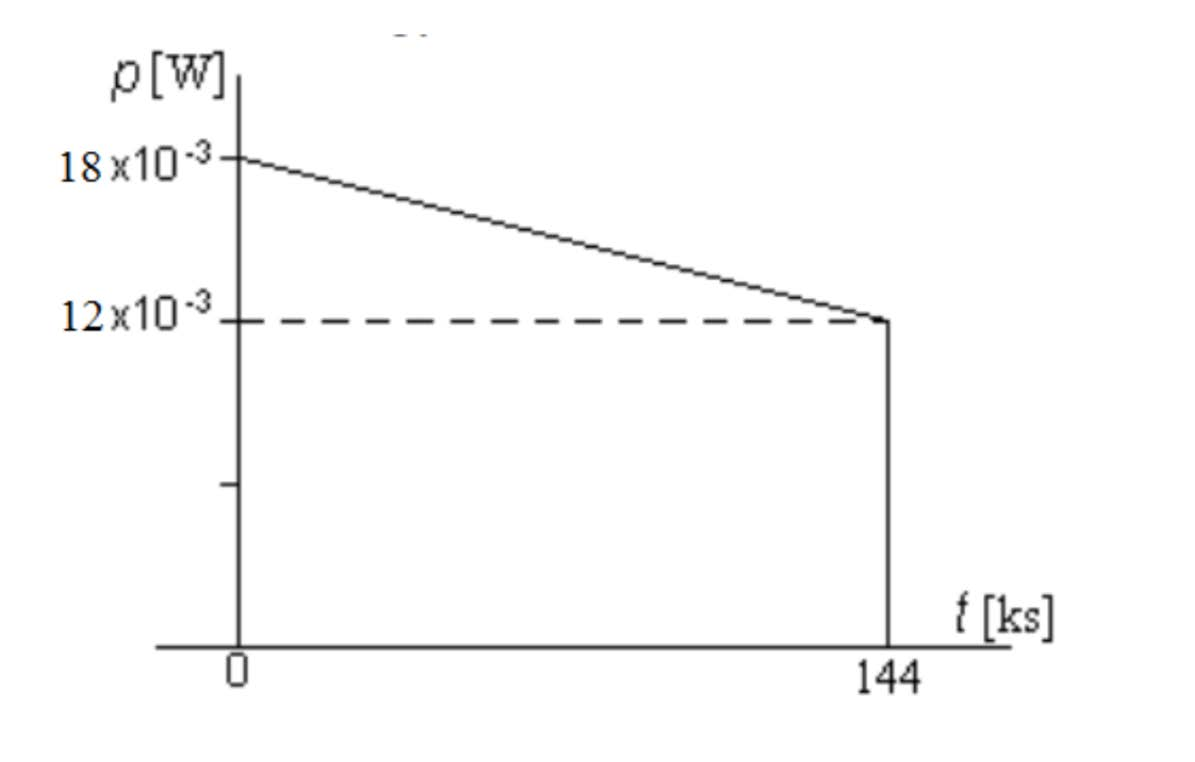
\includegraphics[width=0.4\textwidth]{s1-1.png} 
        \end{center}
    Note that in constructing the plot above, we used the fact that 40 hr = 144,000 s = 144 ks
    \vspace{-1em}
        \begin{align*}%公式居中且左对齐,align带上*号,表示省略掉公式后的编号
        p(0) &=(1.5)(12 \times 10^{-3})=18 \times 10^{-3} W \\
        p(144 ks) &=(1)(12 \times 10^{-3})=12 \times 10^{-3} W \\
        w &=(12 \times 10^{-3})(144 \times 10^3)+\frac{1}{2}(18 \times 10^{-3} - 12 \times 10^{-3})(144 \times 10^3)=2160 J 
        \end{align*}
    \end{quote}
    
    \item (15 points) \uline{Problem 2.7} of the textbook (p71), while the left and middle independent voltage sources are changed from 50 V and 80 V to 100 V and 200 V, respectively.
    \begin{quote}
        
    
    Ans:\\
        The interconnection is valid. In the middle branch, the value of the current $i_{\Delta}$ must be -25 A, since the 25 A current source supplies current in this branch in the direction opposite the direction of the current $i_{\Delta}$. Therefore, the voltage supplied by the dependent voltage source in the left hand branch is $6 (-25) = -150$ V. This gives a voltage drop from the top terminal to the bottom terminal in the left hand branch of $100 -(-150) = 250$ V. And the voltage drop between these same terminals in the right hand branch is 250 V, due to the voltage source in that right branch. Therefore, the interconnection is valid.
    \end{quote}
    \item (20 points) \uline{Problem 2.17} of the textbook (p73), while the resistor in (c) is changed from 400 $\Omega$ to 100 $\Omega$.
    \begin{quote}
        
        
        Ans:\\
        a). Begin by constructing a plot of voltage versus current:
        \begin{center}
            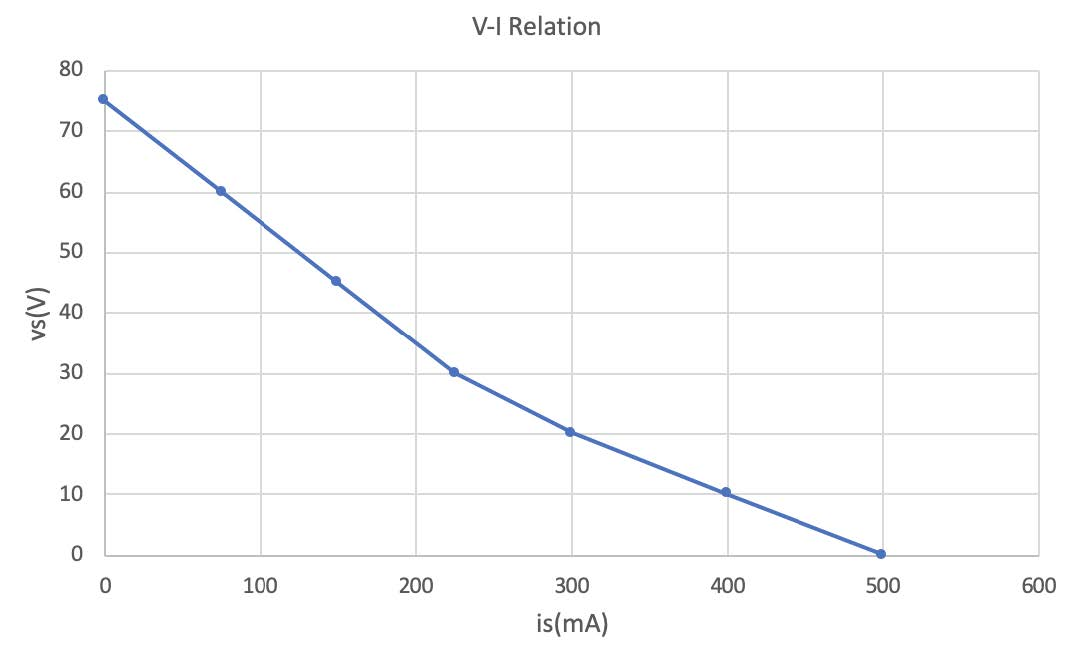
\includegraphics[width=0.4\textwidth]{s1-3.png} 
        \end{center}
        b). Since the plot is linear for $0 \leq i_s \leq 225$ mA amd since R = $\Delta v/\Delta i$, we can calculate R from the plotted values as follows:
        \[R=\dfrac{\Delta v}{\Delta i} = \dfrac{75-30}{0.225 - 0}=\dfrac{45}{0.225}=200 \Omega \]
        We can determine the value of the ideal voltage source by considering the value of $v_s$ when $i_s = 0$. When there is no current, there is no voltage drop across the resistor, so all of the voltage drop at the output is due to the voltage source. Thus the value of the voltage source must be 75 V. The model, valid for $0 \leq i_s \leq 225$ mA, is shown below:
            \begin{center}
                \begin{circuitikz}[american voltages, american currents, american resistors]
                    \draw (0, 0) to[R, -, l=$200 \Omega$] (-3,0) to[V, -, l=$75V$] (-3, -3) to [short, -] (0, -3);
                    
                \end{circuitikz}
            \end{center}
        c). The circuit is shown below:
        \begin{center}
            \begin{circuitikz}[american voltages, american currents, american resistors]
                \draw (0, 0) to[R, -, l=$200 \Omega$] (-3,0) to[V, -, l=$75V$] (-3, -3) to [short, -] (0, -3) to[R,-, l=$100\Omega$](0,0);
                \draw[->] (-0.5, 0.2)  to (0, 0.2);
                \node at (-0.2, 0.35){i};
            \end{circuitikz}
        \end{center}
        Write a KVL equation in the clockwise direction, starting below the voltage source. Use Ohm’s law to express the voltage drop across the resistors in terms of the current $i$:
        \[-75+200i+100i=0, \qquad so \qquad 300i =75 V\]
        Thus,\begin{center}
            $i=\frac{75}{300}=250 mA$ \\
        \end{center} 
        
        d). The circuit is shown below:
        \begin{center}
            \begin{circuitikz}[american voltages, american currents, american resistors]
                \draw (0, 0) to[R, -, l=$200 \Omega$, f<_=$i$] (-3,0) to[V, -, l=$75V$] (-3, -3) to [short, -] (0, -3) to[-, short](0,0);
               % \draw[->] (-0.5, 0.2)  to (0, 0.2);
               % \node at (-0.2, 0.35){i};
            \end{circuitikz}
        \end{center}
    Write a KVL equation in the clockwise direction, starting below the voltage source. Use Ohm’s law to express the voltage drop across the resistors in terms of the current $i$:
     \[-75+200i=0, \qquad so \qquad 200i =75 V\] %underfull是说该处排版内容太稀疏了
    Thus,
    \begin{center}
        $i=\frac{75}{200}=375 mA$ \\
    \end{center}
    
     e). The short circuit current can be found in the table of values (or from the plot) as the value of the current is when the voltage $v_s = 0$. Thus, $i_{sc} = 500 mA$ (from table) \\
     
     f). The plot of voltage versus current constructed in part (a) is not linear (it is piecewise linear, but not linear for all values of $i_s$). Since the proposed circuit model is a linear model, it cannot be used to predict the nonlinear behavior exhibited by the plotted data.
     
    \end{quote}
    \item (10 points) \uline{Problem 2.20} of the textbook (p73), while the current ia is changed from 2 mA to 5 mA.
    \begin{quote}
        
        
        Ans:\\
        a). Use KVL for the right loop to calculate the voltage drop across the right-hand branch $v_0$. This is also the voltage drop across the middle branch, so once $v_0$ is known, use Ohm’s law to calculate $i_0$:
        \[v_0=5000i_a + 4000i_a + 3000i_a =12000(0.005)=60V\]
        \[i_0=\frac{60}{2000}=30mA\]
        b). $i_g=i_a+i_0=35 mA$
        c). The voltage drop across the source is $v_0$,  seen by writing a KVL equation for the left loop. \\
        Thus, $p_g=-v_0 i_g = -(60)(0.035)=2.1 W$ \\
        Thus the source delivers 2.1W.
        
    \end{quote}

    \item (15 points) \uline{Problem 2.25} of the textbook (p74), while the voltage source is changed from 240 V to 300 V and the 45-$\Omega$ to 180-$\Omega$ resistances are changed to 50 $\Omega$ and 170 $\Omega$, respectively.
  \begin{quote}
     
    \begin{center}
        \begin{circuitikz}[american voltages, american currents, american resistors]
            \draw (0, 0) to[short, *- ] (-3,0) to[V, -*, l^=$300V$] (-3, 3) to [R, -*, l^=R, f_=$i_e$] (0, 3) to[-, R, l=$170\Omega$, f=$i_a$](0,0) to[R, -, l=$18\Omega$] (3, 0) to[R, -*, l^=$12\Omega$, f<_=$i_d$, v<=$60 V$] (3, 3) to[-, short] (3, 4.5) to[R, -, l=$50\Omega$, f<_=$i_b$] (-3, 4.5) to (-3, 3);
            
            \draw (0, 3) to[R, -, l=$10\Omega$, f=$i_c$] (3,3);
            \node at (-3.2, 3){a};
            \node at (0, 3.3){b};
            \node at (3.2, 3){c};
            \node at (0, -0.3){d};
        \end{circuitikz}
    \end{center}
    \begin{align*}%公式居中且左对齐,align带上*号,表示省略掉公式后的编号
        &i_d=60/12=5A; &v_{cd}=60+18(5)=150V\\
        &v_{ac} + v_{cd} = 300; &v_{ac}=300-150=150V \\
        &i_b=v_{ac}/50=3A; &i_c=i_d-i_b=2A \\
        &v_{bd}=10i_c + v_{cd}=170V;&i_a=v_{bd}/170=1A\\
        &i_e=i_a+i_c=3A & \\
        &v_{ab}+v_{bd}=300;&v_{ab}=300-170=130V\\
        &R=v_{ab}/i_e=130/3=43.3\Omega &       
    \end{align*}
   \end{quote}
    \item (15 points) \uline{Problem 2.30} of the textbook (p75), while the left voltage source is changed from 100 V to 125 V.
    \begin{quote}
        a).
        \begin{align*}
        &125-20i_{\sigma} + 18i_{\Delta}=0\\
        &-18i_{\Delta}+5i_{\sigma} +40i_{\sigma}=0; 18i_{\Delta}=45i_{\sigma}\\
        &125-20i_{\sigma} + 45i_{\Delta}=0\\
        &So, i_{\sigma}=5A \qquad and \qquad i_{\Delta}=12.5A \\
        &v_0=40i_{\sigma}=200V
        \end{align*}
        b).
        $i_g = $ 
        current out of the positive terminal of the 125 V source
        $v_d = $ voltage drop across the $8_{\Delta}$ source
        \begin{align*}
        i_g&= i_{\Delta}+i_{\sigma}+8i_{\Delta}=9i_{\Delta}+i_{\sigma}=117.5A\\
        v_d&=200-20=180V\\
        \sum P_{gen} & = 125i_g+20i_{\sigma}i_g=125(117.5)+20(5)(117.5)=26437.5W\\
        \sum P_{diss} & = 18(i_{\Delta})^2+5i_{\sigma}(i_g-i_{\Delta})+40(i_{\sigma})^2 + 8i_{\Delta}(v_d+20)\\
        &=(18)(12.5)^2+25(117.5-12.5)+(40)(25)+(8)(12.5)(200) \\
        &=26437.5W=\sum P_{gen}
        \end{align*}
    \end{quote}
    \item (10 points) \uline{Problem 2.34} of the textbook (p76), while the resistance of the trunk is changed from 50 $\Omega$ to 150 $\Omega$.
    \begin{quote}
        a). From the simplified circuit model, using Ohm’s law and KVL :
        \[400i + 150i+200i-250=0; i=250/750=333 mA \]
        This current is nearly enough to stop the heart, according to Table 2.1, so a warning sign
        should be posted at the 250 V source.\\
        b). The closest value from Appendix H to 400 is 390; The closest value from Appendix H to 150 is exactly 150. There are two possibilities for replacing the 200 resistor with a value from Appendix H – 180 and 220. We calculate the resulting current for each of these possibilities, and determine which current is closest to 333 mA:
        \[390i+150i+180i-250=0;i=250/720=347mA\]
        \[390i+150i+220i-250=0;i=250/760=329mA\]
        Therefore, choose the 220 resistor to replace the 200 resistor in the model.
    \end{quote}
\end{enumerate}
\end{document}
